\documentclass[12pt]{article}

\usepackage{fontawesome}
\usepackage{hyperref}
\usepackage{xurl}
\usepackage{graphicx}
\usepackage{float}
\usepackage[tagged, highstructure]{accessibility}
\usepackage{bookmark}
\usepackage{enumitem}

\hypersetup{
    colorlinks=false,
    pdfborder={0 0 0},
    pdftitle={Lab Template},
    pdfauthor={Adrianna Holden-Gouveia},
    pdfsubject={Advanced Data - Lab Assignment},
    pdflang={en-US},
    pdfkeywords={lab assignment, template}
}

% Configure PDF bookmarks for navigation
\bookmarksetup{
    numbered,
    open,
}

% Configure list spacing for better accessibility
\setlist{nosep}



\title{Lab Template}
\author{
        Adrianna Holden-Gouveia \\
        Website: \href{https://aholdengouveia.name}{aholdengouveia.name}\\ 
        \date{\vspace{-5ex}}
        %Email: \href{mailto:admin@aholdengouveia.name}{admin@aholdengouveia.name} \\
%        \faLinkedin{: aholdengouveia} \\
        \faGithub {: aholdengouveia} \\
        %\faTwitter {: aholdengouveia} \\
        }

%S\date{\today}


\begin{document}    

\maketitle

%\begin{abstract}
%This is a template for Linux Administration Lab work
%\end{abstract}
%\tableofcontents


\section*{Accessibility Notice}
This document is also available in HTML format at:

Link: \href{https://aholdengouveia.name/AdvData/labs/labtemplate.html}{\textbf{\nolinkurl{https://aholdengouveia.name/AdvData/labs/labtemplate.html}}}

The HTML version provides enhanced accessibility features including keyboard navigation, screen reader support, responsive design, dark mode support, and high contrast options.

\section*{Request}
\noindent\textbf{Request:} DATA-\#\#\#\# (a random number)\\
\textbf{Requested by:} Who is asking, such as a manager at your company\\
\textbf{Data:} Which data set or database

\section*{Background}
A few sentences on the situation at the company, and why this request matters.

\section*{Learning Outcomes}
By the end of this lab, you will be able to:
\begin{itemize}
    \item Outcome 1, starting with a measurable verb such as write, create, evaluate, or explain
    \item Outcome 2 (no more than 4 outcomes)
\end{itemize}
\section*{Lab Instructions}
Books are my example data only. Students use their own data set from the Introduction to Data lab.

\subsection*{Screenshots}
Several parts of this lab ask for a screenshot. Each screenshot should have your name, term, and year.  One of the easiest ways to do that is make a text document with your name and term/year on your computer and save it to use all term. Any screenshots that don't include this information won't be counted.

\begin{figure}[H]
    \centerline{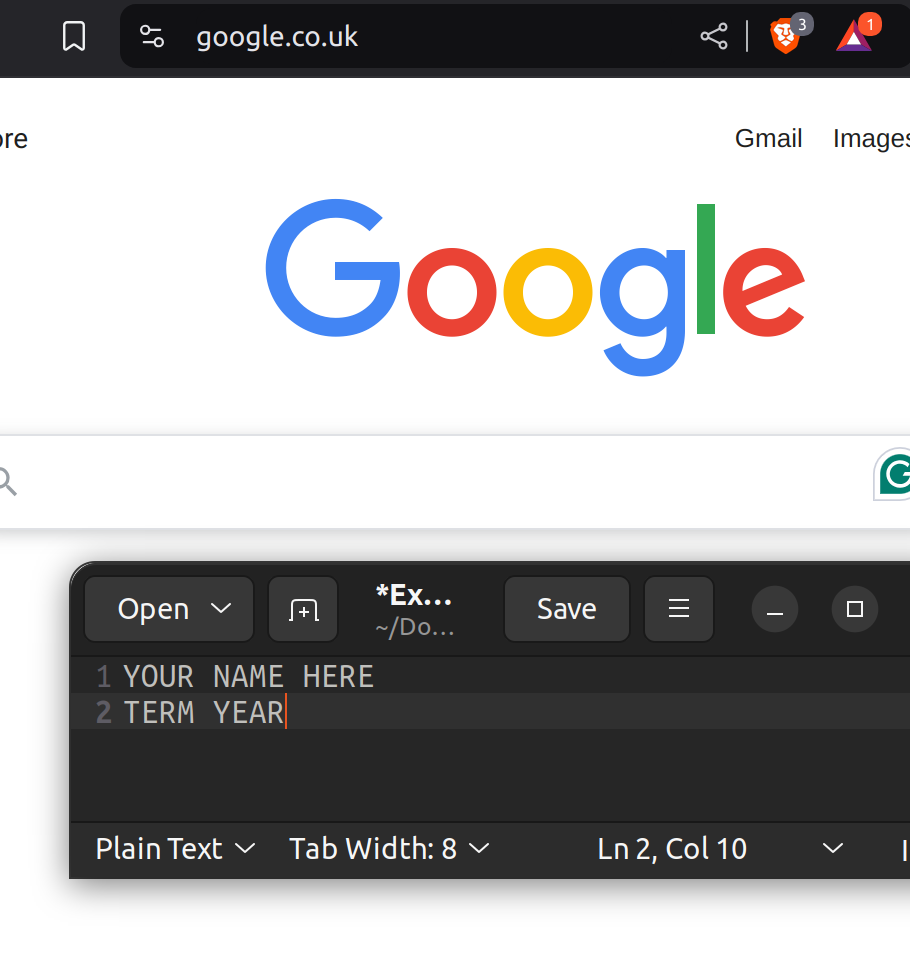
\includegraphics[scale=.2]{ExampleScreenshot.png}}
    \caption{This is an image of what each of your screenshots should look like}
    \alt{Example screenshot: a web browser showing the Google home page, with a small text editor window in front of it that says YOUR NAME HERE and TERM YEAR}
\end{figure}

\subsection*{Part 1: Title}
\begin{enumerate}
    \item 1
    \item 2
    \item 3
\end{enumerate}

\section*{Acceptance Criteria}
This request is done when:
\begin{itemize}
    \item Something you can check is done
    \item Another one
\end{itemize}

\section*{Deliverables}
One file that includes:
\begin{itemize}
    \item Part 1: ...
\end{itemize}

Audience: who will read this, and what they already know.

\section*{Resources}
References, a video, a PowerPoint and some notes are available at my website
Link: \href{https://www.aholdengouveia.name}{\textbf{\nolinkurl{https://www.aholdengouveia.name}}}

% ============================================================
% EXAMPLE: Accessible Table (if needed)
% Uncomment and modify the lines below to add a table
% This ensures proper screen reader support
% ============================================================
%\begin{table}[h]
%\caption{Command Options}
%\begin{tabular}{|l|l|}
%\hline
%\textbf{Option} & \textbf{Description} \\
%\hline
%-F & Field separator \\
%\hline
%-v & Variable assignment \\
%\hline
%\end{tabular}
%\end{table}

\end{document}